\mode*
\lecture[Tutorial]{A Very Brief Internet Tutorial (II)}{tutorial}
%\mode<article>{\clearpage}

\subsection{TCP/IP Overview}

\paragraph{Historical}

  The ARPANET was a research network sponsored by the DoD (U.S. Department of
  Defense). ...  When satellite and radio networks were added later, the existing
  protocols had trouble interworking with them, so a new reference architecture was
  needed. Thus, \emph{from nearly the beginning, the ability to connect multiple networks in
    a seamless way was one of the major design goals}.  This architecture later became
  known as the TCP/IP Reference Model, after its two primary protocols. \citetitle[Sec.~1.4.2,
  \emph{The TCP/IP Reference Model}]{tanenbaum2011computer}

  Given the DoD's worry that some of its precious hosts, routers, and internetwork
  gateways might get blown to pieces at a moment's notice by an attack from the Soviet
  Union, another major goal was that the network be able to survive loss of subnet
  hardware, without existing conversations being broken off. In other words, \emph{the DoD
    wanted connections to remain intact as long as the source and destination machines
    were functioning, even if some of the machines or transmission lines in between were
    suddenly put out of operation}. Furthermore, since applications with divergent
  requirements were envisioned, ranging from transferring files to real-time speech
  transmission, a flexible architecture was needed.


\begin{frame}{{\tcpip} Overview}{Basic Structure}
  \begin{minipage}{.4\linewidth}
    \includegraphics[width=\textwidth]{basic-structure}\label{fig:basic-node}
  \end{minipage}\hfill
  \begin{minipage}{.6\linewidth}
    \begin{enumerate}
    \item Where will an incoming Ethernet frame go?
      \begin{itemize}
      \item[] \texttt{0x0806} {\dejavu ➜} ARP
      \item[] \texttt{0x0800} {\dejavu ➜} IP
      \end{itemize}
    \item Where will an incoming IP packet go?
      \begin{itemize}
      \item[] \texttt{0x06} {\dejavu ➜} TCP
      \item[] \texttt{0x11} {\dejavu ➜} UDP
      \end{itemize}
    \item Where will an incoming transport message (UDP datagram, TCP segment) go?
      \begin{center}
        \begin{tblr}{colspec={cccc},hline{1,Z},rowsep=0pt,%
            row{1}={font=\small},row{2}={font=\ttfamily\small},}
          HTTP&FTP&SSH&SMTP\\
          80&21/20&22&25\\
        \end{tblr}
      \end{center}
    \end{enumerate}
  \end{minipage}
\end{frame}

\subsection{Terminology}
  
\begin{frame}{The Name Of A Unit Of Data}
  \mode<beamer>{\vspace*{-5em}}
  \begin{minipage}{.47\linewidth}
    \begin{itemize}
    \item[APP] Application message
    \item[TRANS] TCP segment; UDP datagram
    \item[NET] IP packet
    \item[LINK] Ethernet frame
    \end{itemize}
  \end{minipage}\hfill
  \begin{minipage}{.5\linewidth}
    \mode<beamer>{ 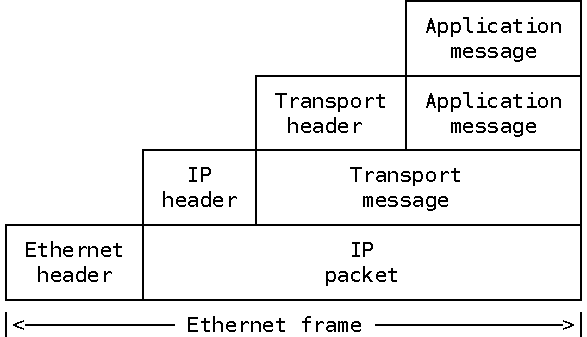
\includegraphics[width=\columnwidth]{encap} }%
    \mode<article>{ 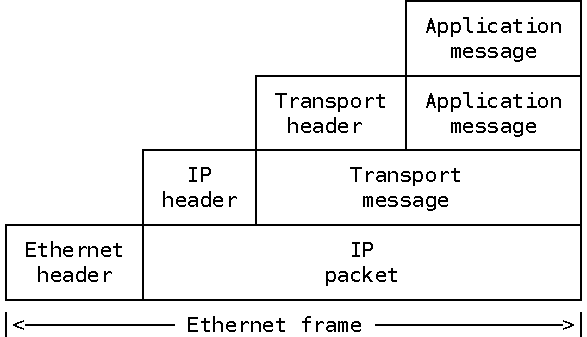
\includegraphics[width=.7\columnwidth]{encap} }
  \end{minipage}
  \mode<beamer>{
    \begin{tikzpicture}[remember picture, overlay]
      \node [red,opacity=.3,anchor=center,yshift=5mm,scale=.4] at (current page.south)%
      {\includegraphics{indirect-routing-2}};
    \end{tikzpicture}}
\end{frame}

\subsection{Ethernet}
  
\begin{frame}\mode<beamer>{\frametitle{Ethernet}}
  \begin{center}
    \mode<beamer>{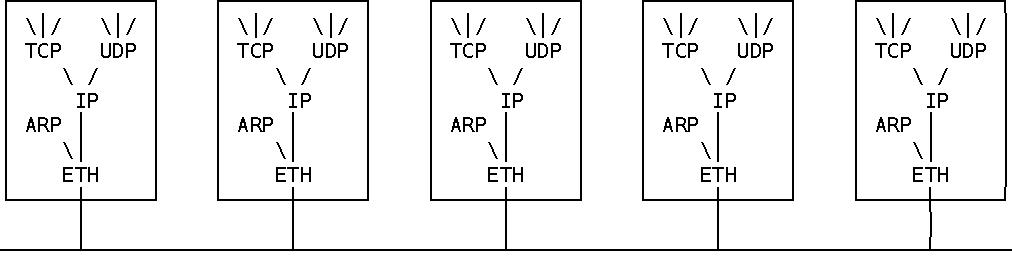
\includegraphics[width=\textwidth]{eth}}%
    \mode<article>{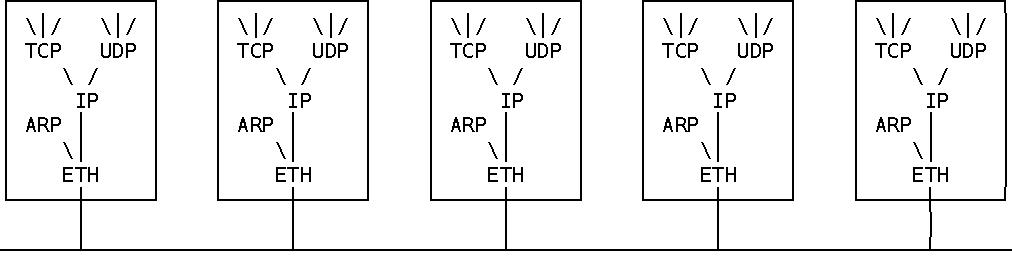
\includegraphics[width=.6\textwidth]{eth}}
  \end{center}
  \begin{enumerate}
  \item Frame format?
  \item Address format?
  \item Broadcast address?
  \item CSMA/CD?
  \end{enumerate}
\end{frame}

\begin{frame}{Ethernet Frame}
  \begin{center}
    \mode<beamer>{ 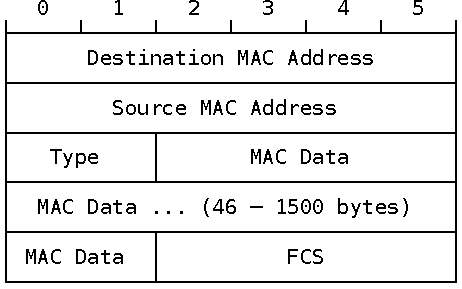
\includegraphics[width=.65\textwidth]{ethhdr} }%
    \mode<article>{ 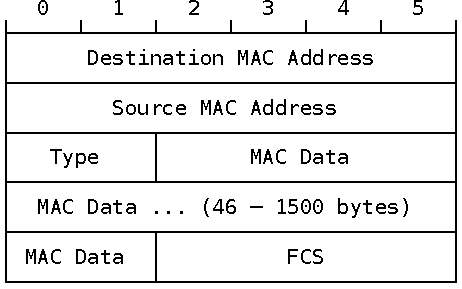
\includegraphics[width=.3\textwidth]{ethhdr} }
  \end{center}
\end{frame}

\begin{frame}{Examples}
  \begin{iblock}{Unicast, carrying an IP packet}
    \centering
    \mode<beamer>{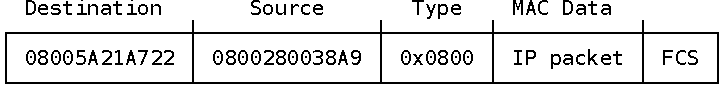
\includegraphics[width=.9\textwidth]{ethframe3}}%
    \mode<article>{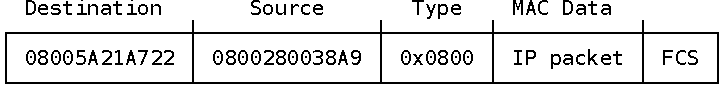
\includegraphics[width=.6\textwidth]{ethframe3}}
  \end{iblock}
  \begin{iblock}{Unicast, carrying an ARP packet}
    \centering
    \mode<beamer>{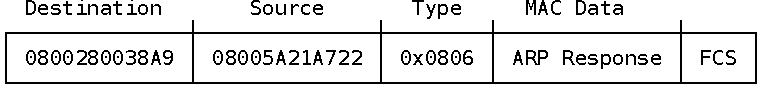
\includegraphics[width=.9\textwidth]{ethframe2}}%
    \mode<article>{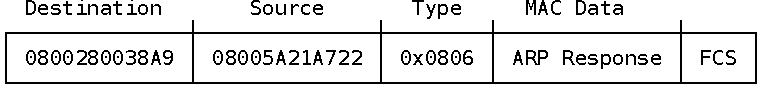
\includegraphics[width=.6\textwidth]{ethframe2}}
  \end{iblock}
  \begin{iblock}{Broadcast, carrying an ARP packet}
    \centering
    \mode<beamer>{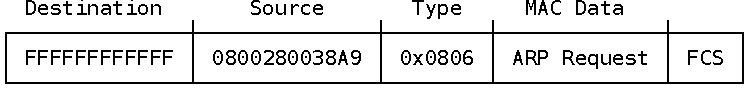
\includegraphics[width=.9\textwidth]{ethframe}}%
    \mode<article>{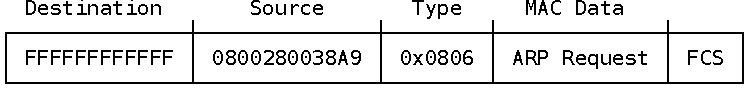
\includegraphics[width=.6\textwidth]{ethframe}}
  \end{iblock}
\end{frame}

\begin{description}
\item[CSMA/CD] CSMA/CD is the communication protocol used by devices in the same Ethernet
  when they talk to each other.
  \begin{itemize}
  \item \emph{Carrier Sense} means every device in the Ethernet can detect whether the
    carrier is busy. Carrier, the media used for carrying electric signals, is the Ethernet cable;
  \item \emph{Multiple Access} means every device has equal chance of using the carrier
    for data transmission ;
  \item \emph{Collision Detection} means if more than one devices trying to transmit
    data at the same time, they can detect this collision, and wait for a random (but
    short) period before trying to transmit again.
  \end{itemize}
  See \citetitle[Sec. 3.1]{rfc1180} for a human analogy.
\end{description}

\subsubsection{Bridge, Switch}

\begin{frame}\mode<beamer>{\frametitle{Bridge, Switch}}
  \begin{description}
  \item[Bridge] connects multiple network segments at the data link layer (layer 2)
  \item[Switch] a multi-port bridge
  \end{description}
  \begin{columns}[b]
    \begin{column}{.45\linewidth}
      \begin{iblock}{Transparent bridging}
        Uses a forwarding database to send frames across network segments
        \begin{itemize}
        \item Learning
        \item Flooding
        \item Forwarding
        \item Filtering
        \item Aging
        \end{itemize}
      \end{iblock}
    \end{column}
    \begin{column}{.55\linewidth}
      \mode<beamer>{
\includegraphics[width=\textwidth]{switch}}%
      \mode<article>{
\includegraphics[width=.5\textwidth]{switch}}%
    \end{column}
  \end{columns}
\end{frame}

\paragraph{Transparent bridging}

\begin{itemize}
\item \url{https://en.wikipedia.org/wiki/Bridging_(networking)}
\item \url{https://www.oreilly.com/library/view/ethernet-switches/9781449367299/ch01.html}
\end{itemize}

Ethernet switches are designed so that their operations are invisible to the devices on
the network, which explains why this approach to linking networks is also called
\emph{transparent bridging}. “Transparent” means that when you connect a switch to an Ethernet
system, no changes are made in the Ethernet frames that are bridged. The switch will
automatically begin working without requiring any configuration on the switch or any
changes on the part of the computers connected to the Ethernet network, making the
operation of the switch transparent to them.

\paragraph{Two methods in forwarding frames}
\begin{itemize}
\item \url{https://www.orbit-computer-solutions.com/understanding-how-switches-forwards-frames-in-ethernet-network/}
\end{itemize}
\begin{description}
\item[Store-and-forward switching:] Receive and store frame, check for errors and forward
  it towards its destination or discard if error is found. (Bandwidth efficient)
\item[Cut-through switching:] Works on the frame soon as it is received, even if the
  transmission is not complete. Don't check for errors, lookup destination port and
  forward. (Faster)
\end{description}
Most switches are configured to perform cut-through switching on a per-port basis until a
user-defined error mark is reached and then they automatically change to
store-and-forward. When the error rate falls below the threshold, the port automatically
changes back to cut-through switching.

\begin{frame}{Switch Loop}
  \begin{itemize}
  \item[{\Large ☺}] Redundancy --- Eliminating the single point of failure
  \item[{\Large \textcolor{red}{☹}}] Broadcast storm --- Resulting in potentially severe network congestion
  \end{itemize}
  \centering
  \mode<beamer>{ 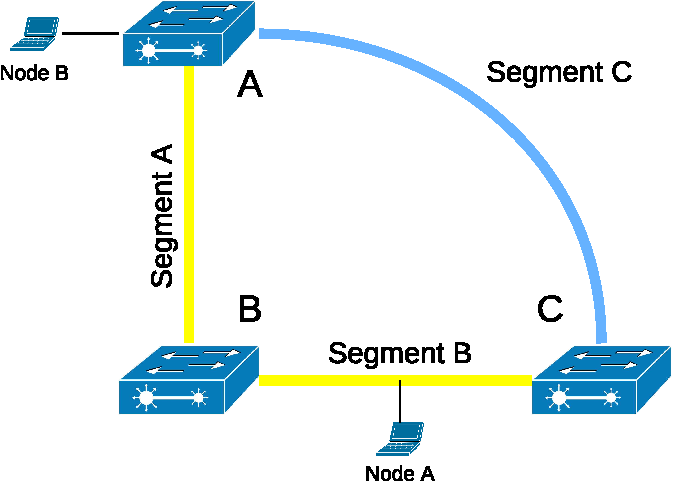
\includegraphics[width=.6\textwidth]{bcast-storm} }%
  \mode<article>{ 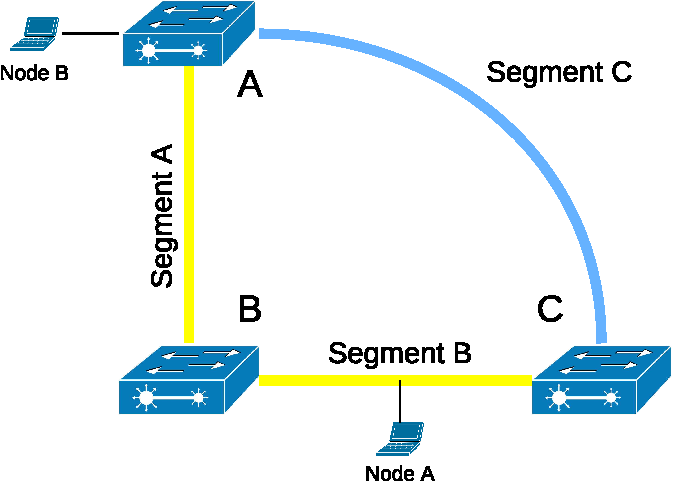
\includegraphics[width=.3\textwidth]{bcast-storm} }
\end{frame}

\begin{itemize}
\item \url{https://computer.howstuffworks.com/lan-switch13.htm}
\end{itemize}

\begin{enumerate}
\item A packet is sent from Node B to Node A;
\item Switch A has no knowledge of Node A, it floods Seg A and Seg C;
\item Assuming both Switch B and Switch C have no record of Node A. They will:
  \begin{enumerate}
  \item Update their forwarding table respectively by adding a record of Node B;
  \item Flood Seg B looking for Node A.
  \end{enumerate}
\item Both Switch B and Switch C will see this packet. Then,
  \begin{enumerate}
  \item Switch B will flood Seg A; Switch C will flood Seg C, because they still don't
    know who Node A is.
  \item Update their forwarding table respectively by adding a record
    of Node A \emph{only if Node A is up and respond to the received message}.
  \end{enumerate}
\item Switch A gets the floods from both Seg A and Seg C, and floods it out again.
\end{enumerate}

\begin{frame}
  \begin{description}
  \item[Spanning Tree Protocol (STP)] is a network protocol that ensures a loop-free
    topology for any bridged Ethernet local area network.
  \end{description}
  \begin{center}
    \mode<beamer>{ 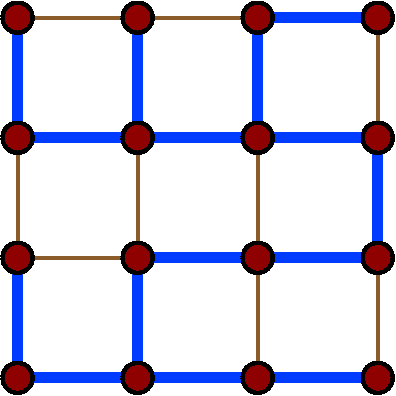
\includegraphics[width=.4\textwidth]{spanning-tree} }%
    \mode<article>{ 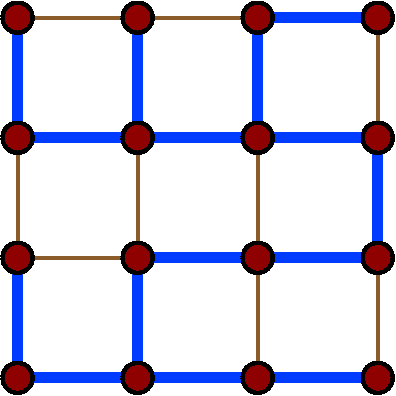
\includegraphics[width=.1\textwidth]{spanning-tree} }
  \end{center}
\end{frame}

\begin{frame}<beamer>{Algorhyme}
  \begin{minipage}{.55\linewidth}
    \begin{verse}
      I think that I shall never see\\
      A graph more lovely than a tree.\\[1ex]
      A tree whose crucial property\\
      Is loop-free connectivity.\\[1ex]
      A tree that must be sure to span\\
      So packets can reach every LAN.\\[1ex]
      First, the root must be selected.\\
      By ID, it is elected.\\[1ex]
      Least cost paths from root are traced.\\
      In the tree, these paths are placed.\\[1ex]
      A mesh is made by folks like me\\
      Then bridges find a spanning tree.\\[1ex]
    \end{verse}
    \begin{flushright}{\footnotesize --- Radia Perlman\hspace{3em}}\end{flushright}    
  \end{minipage}
  \begin{minipage}{.4\linewidth}
    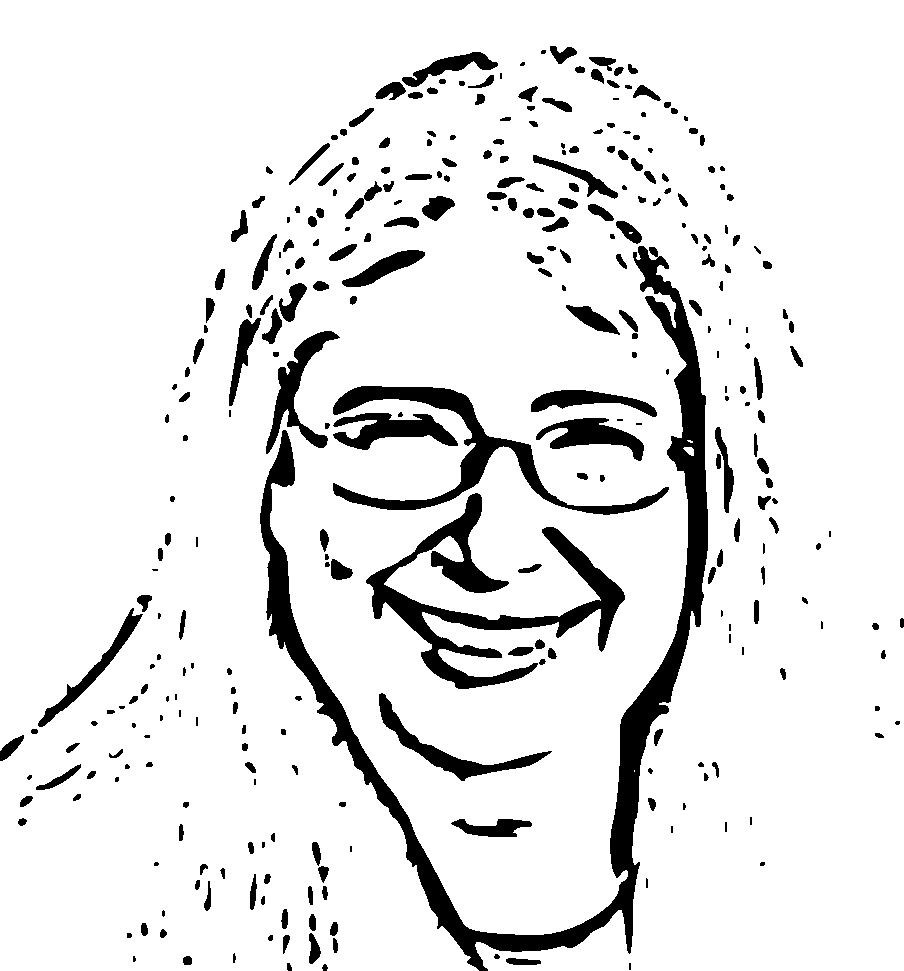
\includegraphics[width=\textwidth]{radia}
  \end{minipage}
\end{frame}

\paragraph{Algorhyme}\ \\

\begin{minipage}{.5\linewidth}
  \begin{verse}
    I think that I shall never see\\
    A graph more lovely than a tree.\\[1ex]
    A tree whose crucial property\\
    Is loop-free connectivity.\\[1ex]
    A tree that must be sure to span\\
    So packets can reach every LAN.\\[1ex]
    First, the root must be selected.\\
    By ID, it is elected.\\[1ex]
    Least cost paths from root are traced.\\
    In the tree, these paths are placed.\\[1ex]
    A mesh is made by folks like me\\
    Then bridges find a spanning tree.\\[1ex]
  \end{verse}
  \begin{flushright}{\footnotesize --- Radia Perlman\hspace{3em}}\end{flushright}
\end{minipage}
\begin{minipage}{.2\linewidth}
  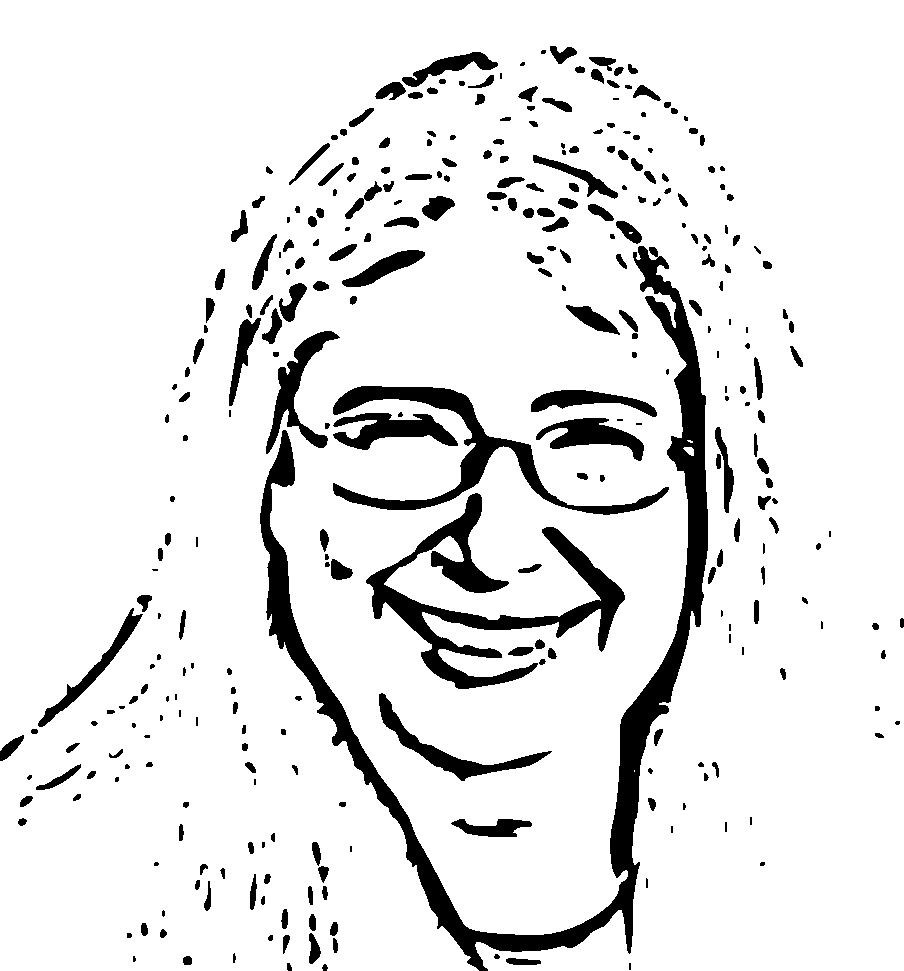
\includegraphics[width=\textwidth]{radia}
\end{minipage}

\begin{itemize}
\item \url{https://en.wikipedia.org/wiki/Radia_Perlman}
\end{itemize}

See also: \citetitle{web:switch, web:tb, wiki:stp}

\begin{frame}{Ethernet References}
  \begin{refsection}
    \nocite{wiki:ethernet,wiki:ethframe,wiki:csmacd,rfc1042,wiki:switch,
      wiki:lanswitching} \printbibliography[heading=none]
  \end{refsection}
\end{frame}

\subsection{ARP}

\begin{frame}\mode<beamer>{\frametitle{ARP}}
  \begin{description}
  \item[ARP] Looking up the ARP table to find the destination MAC address.
  \end{description}
  \begin{minipage}{.5\linewidth}
    \begin{iblock}{Example ARP table}
      {\centering
        \begin{tblr}{colspec={lr},hline{1,2,Z},row{2-Z}={font=\ttfamily}}
          IP address & Ethernet address\\
          223.1.2.1 & 08-00-39-00-2F-C3\\
          223.1.2.3 & 08-00-5A-21-A7-22\\
          223.1.2.4 & 08-00-10-99-AC-54\\
        \end{tblr}}
    \end{iblock}
  \end{minipage}\quad
  \begin{minipage}{.4\linewidth}
    \includegraphics[width=\textwidth]{basic-structure}
  \end{minipage}
\end{frame}

\begin{frame}{Where does the ARP table come from?}
  \begin{minipage}[t]{.6\linewidth}
    \begin{iblock}{Example ARP Request}
      \begin{tblr}{colspec={lr},hline{1,3,5},rows={font=\small},rowsep=0pt,%
          column{2}={font=\small\ttfamily}%
        }
        Sender IP Address & 223.1.2.1\\
        Sender Eth Address & 08-00-39-00-2F-C3\\
        Target IP Address & 223.1.2.2\\
        Target Eth Address & 00-00-00-00-00-00\\
      \end{tblr}
    \end{iblock}
    \begin{iblock}{Example ARP Response}
      \begin{tblr}{colspec={lr},hline{1,3,5},rows={font=\small},rowsep=0pt,%
          column{2}={font=\small\ttfamily}%
        }
        Sender IP Address &  223.1.2.2\\
        Sender Eth Address & 08-00-28-00-38-A9\\
        Target IP Address &  223.1.2.1\\
        Target Eth Address & 08-00-39-00-2F-C3\\
      \end{tblr}
    \end{iblock}
  \end{minipage}\hfill
  \begin{minipage}[t]{.4\linewidth}
    \begin{iblock}{The updated table}
      \begin{tblr}{colspec={lr},hline{1,2,Z},rowsep=0pt,%
          rows={font=\small},row{2-Z}={font=\small\ttfamily}}
          IP address &Ethernet address\\
          223.1.2.1 & 08-00-39-00-2F-C3\\
          223.1.2.2 & 08-00-28-00-38-A9\\
          223.1.2.3 & 08-00-5A-21-A7-22\\
          223.1.2.4 & 08-00-10-99-AC-54\\
        \end{tblr}
    \end{iblock}
    \vspace*{3ex}
    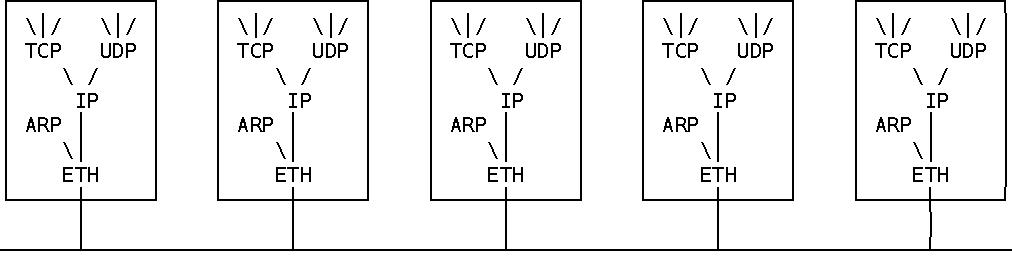
\includegraphics[width=\textwidth]{eth}
  \end{minipage}
\end{frame}

% \begin{frame}{Is Target Info in ARP Reply Necessary?}
%   \begin{itemize}
%   \item Promiscuous mode
%   \item Gratuitous ARP
%   \end{itemize}
% \end{frame}

\begin{frame}{ARP References}
  \begin{refsection}
  \nocite{wiki:arp, rfc826} \printbibliography[heading=none]
\end{refsection}
\end{frame}

\subsection{IP}

\begin{frame}\mode<beamer>{\frametitle{IP}\framesubtitle{Router}}
  \begin{minipage}{.4\linewidth}
      \mode<beamer>{ \includegraphics[width=\columnwidth]{basic-structure} }%
      \mode<article>{ \includegraphics[width=.7\columnwidth]{basic-structure} }
  \end{minipage}\hfill
  \begin{minipage}{.4\linewidth}
      \mode<beamer>{ 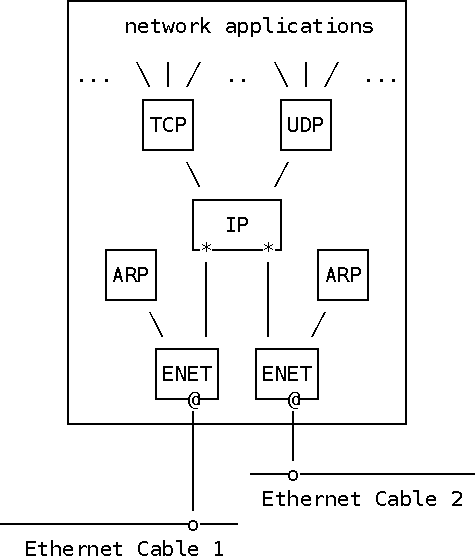
\includegraphics[width=\columnwidth]{basic-structure-2} }%
      \mode<article>{ 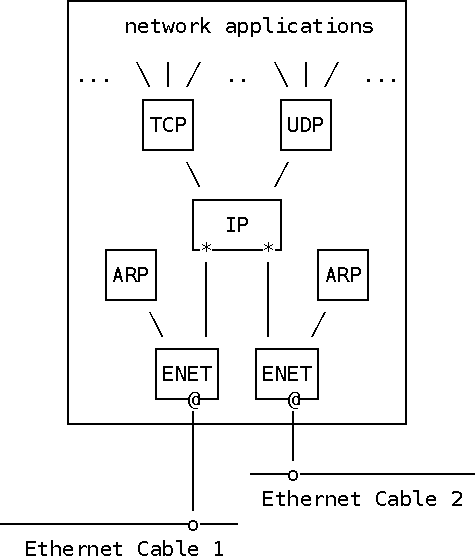
\includegraphics[width=.7\columnwidth]{basic-structure-2} }
      \label{fig:router}
  \end{minipage}
  \begin{description}
  \item[Routing] Find a route in the route table.
  \end{description}
\end{frame}

\begin{frame}{Mail vs. E-mail}
  \begin{tikzpicture}[remember picture, overlay, inner sep=0pt]
    \node at (current page.north west) [anchor=north west, shift={(5mm,-15mm)}, scale=.7]{%
      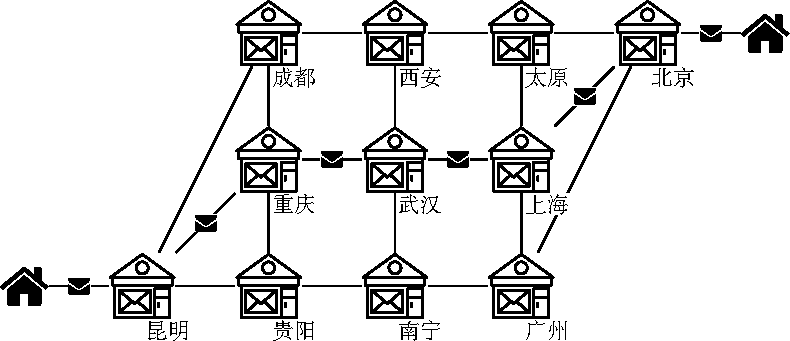
\includegraphics{surfacemailing}
    };

    \node at (current page.south east) [anchor=south east, shift={(-5mm,1cm)}, scale=.9]{
      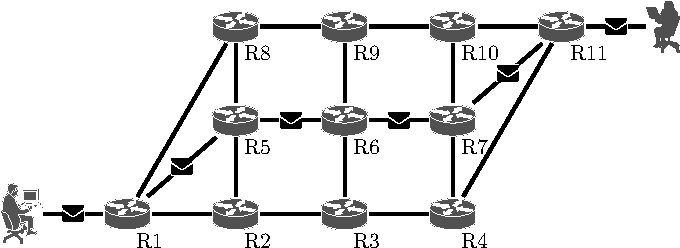
\includegraphics{router4-tikz}
    };
  \end{tikzpicture}
\end{frame}

\begin{frame}{Direct Routing --- IP is overhead}
  \begin{minipage}{.4\linewidth}
    \mode<beamer>{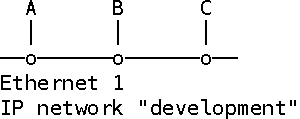
\includegraphics[width=\textwidth]{direct-routing}}%
    \mode<article>{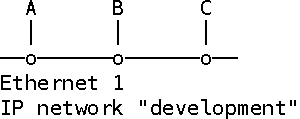
\includegraphics[width=.5\textwidth]{direct-routing}}
  \end{minipage}\qquad
  \begin{minipage}{.4\linewidth}
    \begin{iblock}{A \(\Rightarrow\) B}
      \begin{center}
        \begin{tblr}{colspec={ccc},hline{1,2,Z}}
          Address & Source & Destination \\
          IP      & A      & B           \\
          Eth     & A      & B           \\
        \end{tblr}
      \end{center}
    \end{iblock}
  \end{minipage}
\end{frame}

\begin{frame}{Is IP Necessary?}
  \centering
  \includegraphics[width=.3\textwidth]{without-ip}\quad
  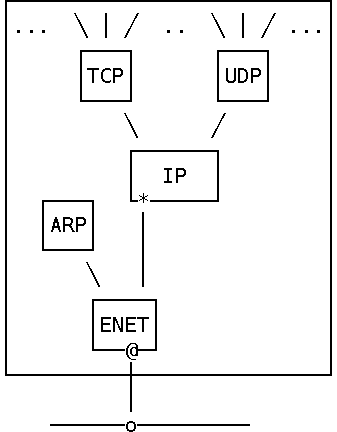
\includegraphics[width=.3\textwidth]{with-ip}\quad
  \includegraphics[width=.3\textwidth]{dual-stack}
\end{frame}

\begin{frame}{Indirect Routing}
  \begin{center}
    \mode<beamer>{ \includegraphics[width=.9\textwidth]{indirect-routing} }%
    \mode<article>{ \includegraphics[width=.5\textwidth]{indirect-routing} }
  \end{center}
  \label{fig:indirect-routing}
  \mode<beamer>{
    \begin{tikzpicture}[remember picture, overlay]
      \node [scale=.5,text opacity=.8,xshift=-60mm, yshift=-40mm] at (current page.center)
      {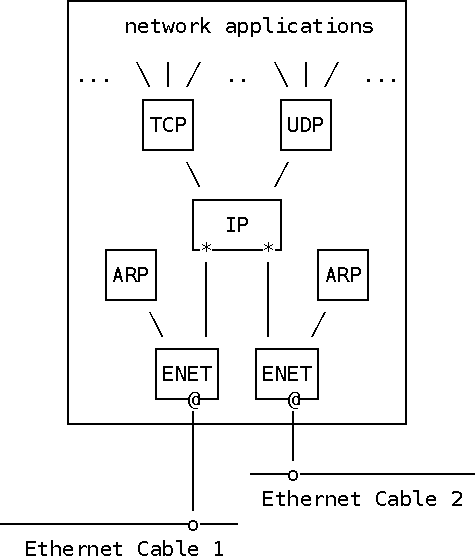
\includegraphics{basic-structure-2}};
    \end{tikzpicture}}
\end{frame}

\begin{frame}{A \(\Rightarrow\) E}
  \begin{center}
    \includegraphics[width=.7\linewidth]{indirect-routing}
  \end{center}
  \begin{minipage}{.45\linewidth}
    \begin{iblock}{Before D}
      \begin{center}
        \begin{tblr}{colspec={ccc},hline{1,2,Z},rowsep=0pt}
          address & source & destination \\
          IP      & A      & E           \\
          Eth     & A      & D           \\
        \end{tblr}
      \end{center}
    \end{iblock}
  \end{minipage}\qquad
  \begin{minipage}{.45\linewidth}
    \begin{iblock}{After D}
      \begin{center}
        \begin{tblr}{colspec={ccc},hline{1,2,Z},rowsep=0pt}
          address & source & destination \\
          IP      & A      & E           \\
          Eth     & D      & E           \\
        \end{tblr}
      \end{center}
    \end{iblock}
  \end{minipage}
\end{frame}

\begin{frame}{IP Module Routing Rules}
  \begin{minipage}{.8\linewidth}
  \begin{enumerate}
  \item For an outgoing IP packet, entering IP from an upper layer, IP must decide
    \begin{itemize}
    \item whether to send the IP packet directly or indirectly, and
    \item IP must choose a lower network interface.
    \end{itemize}
    These choices are made by consulting the route table.
  \item For an incoming IP packet, entering IP from a lower interface, IP must decide
    \begin{itemize}
    \item whether to forward the IP packet or pass it to an upper layer.
    \item If the IP packet is being forwarded, it is treated as an outgoing IP packet.
    \end{itemize}
  \item When an incoming IP packet arrives it is never forwarded back out through the same
    network interface.
  \end{enumerate}
\end{minipage}
\mode<beamer>{
  \begin{tikzpicture}[remember picture, overlay] \node [red,opacity=.3,scale=.45,anchor=east]
    at (current page.east) {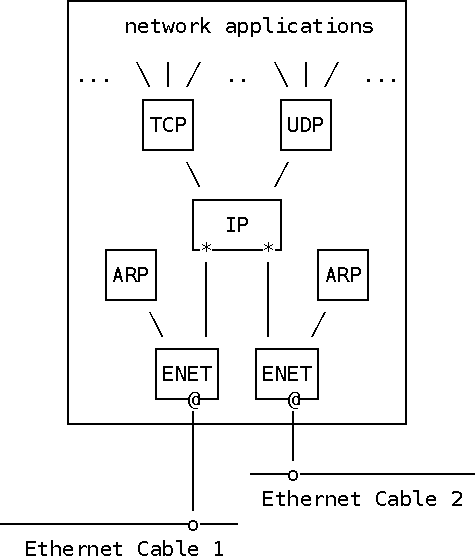
\includegraphics{basic-structure-2}};
  \end{tikzpicture}}
\end{frame}

\begin{frame}{IP Address}
  \centering
  \mode<beamer>{ 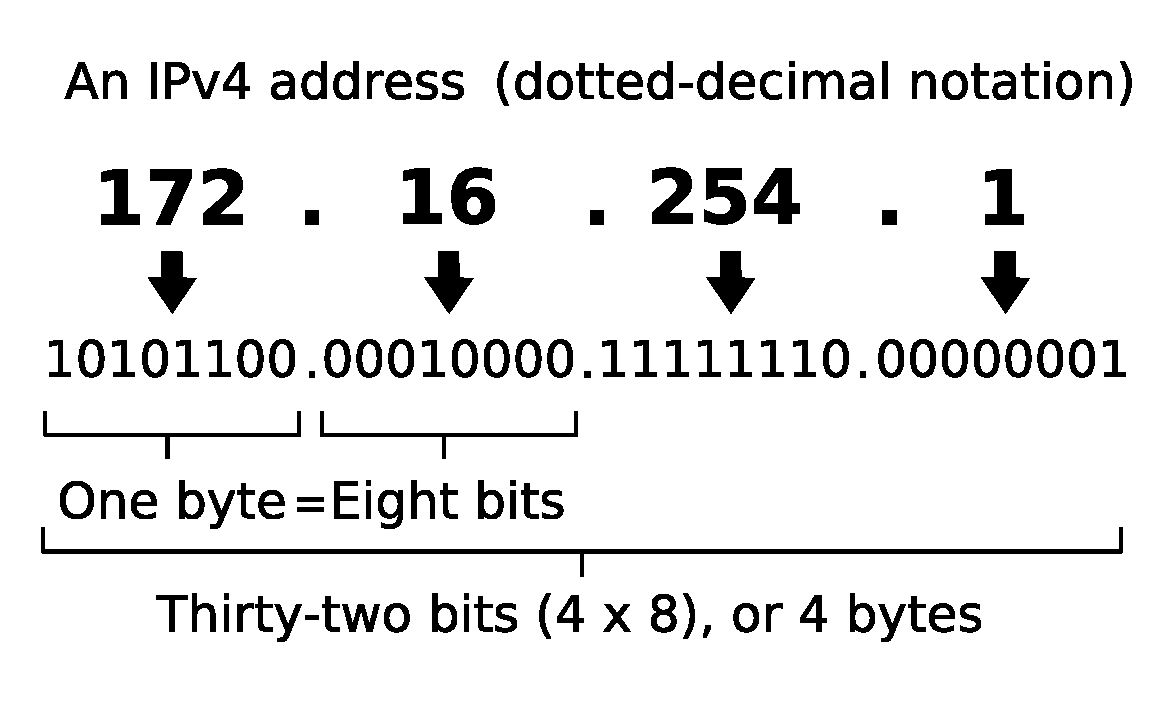
\includegraphics[width=.9\textwidth]{ipv4addr172} }%
  \mode<article>{ 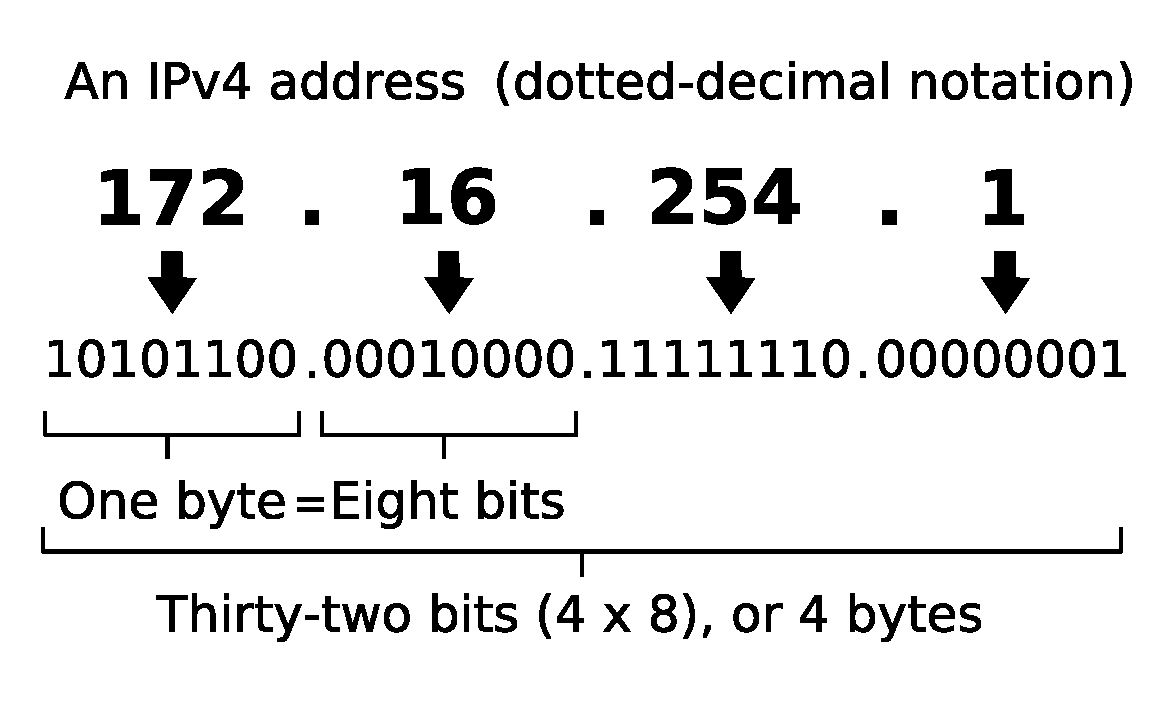
\includegraphics[width=.6\textwidth]{ipv4addr172} }
\end{frame}

\begin{frame}
  \begin{iblock}{Address classes}
    \centering
    \mode<beamer>{ \includegraphics[width=.8\textwidth]{ipv4addr} }%
    \mode<article>{ \includegraphics[width=.6\textwidth]{ipv4addr} }
  \end{iblock}
\end{frame}

\begin{frame}{Network bits?}
  % \begin{iblock}{}%Do maths on the first 8 bits
    \begin{description}
    \item[Dst IP:] \texttt{11000000.10101000.10101000.10101000}
    \end{description}
    
    \begin{center}
      Example route table\\
      \begin{tblr}{colspec={lcc},hline{1,2,Z},%
          row{2,3,4}={font=\ttfamily}, row{1}={c},%
        }
        Destination& Gateway& Iface\\
        \underline{00001010}.00000000.00000000.00000000& *& 1\\
        \underline{10101100.00010000}.00000000.00000000& *& 2\\
        \underline{11000000.10101000.10101000}.00000000& *& 3\\
      \end{tblr}
    \end{center}
  % \end{iblock}
      
  \begin{iblock}{Prefix --- A faster way to decide network bits}
    \centering\label{fig:prefix}
    \mode<beamer>{ 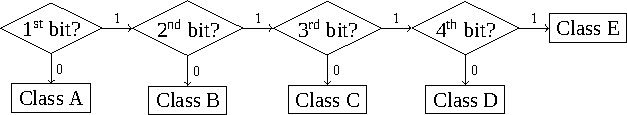
\includegraphics[width=.8\textwidth]{prefix2} }%
    \mode<article>{ 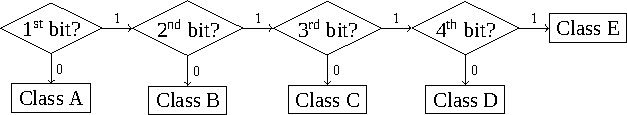
\includegraphics[width=.7\textwidth]{prefix2} }
  \end{iblock}
\end{frame}

\begin{frame}{Special IP Addresses}
  \begin{itemize}
  \item A value of zero in the network field means this network. (source only)
  \item A value of zero in the host field means network address.
  \item \texttt{127.x.x.x} are loopback address.
  \item \texttt{255.255.255.255} is boardcast address.
  \item Private address:{\ttfamily
    \begin{itemize}
    \item 10.x.x.x
    \item 172.16.x.x \char`~{} 172.31.x.x
    \item 192.168.x.x
    \end{itemize}}
  \item CIDR --- Classless Inter-Domain Routing --- An IP addressing scheme that replaces the older
    system based on classes A, B and C.
  \end{itemize}
\end{frame}

See also: \citetitle[\emph{RFC 943}]{rfc943}

\begin{frame}{Names}
  People refer to computers by names, not numbers.
  \begin{iblock}{\texttt{/etc/hosts}}
    \begin{center}
      \begin{tblr}{colspec={lll},rows={font=\ttfamily}}
        127.0.0.1 & localhost&\\
        202.203.132.245 & cs3.swfu.edu.cn & cs3\\
      \end{tblr}
    \end{center}
  \end{iblock}

  \begin{iblock}{\texttt{/etc/networks}}
    \begin{center}
      \texttt{localnet}\qquad \texttt{202.203.132.192}
    \end{center}
  \end{iblock}
\end{frame}

\begin{frame}{IP Route Table}
  \begin{iblock}{Example IP Route Table}
    \begin{center}
      \mode<beamer>{ 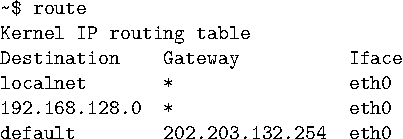
\includegraphics[width=.7\textwidth]{route-table} }%
      \mode<article>{ 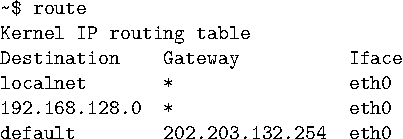
\includegraphics[width=.3\textwidth]{route-table} }
    \end{center}
  \end{iblock}
  \begin{itemize}
  \item[\char`~\$] \texttt{man route}
  \end{itemize}
\end{frame}

\begin{frame}{Direct Routing Details}
  \begin{minipage}{.4\linewidth}
    \mode<beamer>{ \includegraphics[width=.8\textwidth]{direct-routing-2} }%
    \mode<article>{ \includegraphics[width=.6\textwidth]{direct-routing-2} }
  \end{minipage}\quad
  \begin{minipage}{.55\linewidth}
    \begin{iblock}{The route table inside alpha (simplified)}
      \begin{center}
        \begin{tblr}{colspec={llcc},row{2}={font=\ttfamily},hlines}
          network & flag & router & iface\\
          development & direct & * & 1\\
        \end{tblr}
      \end{center}
    \end{iblock}
  \end{minipage}
\end{frame}

\begin{frame}{Homework}
  \centering
  \includegraphics[width=\textwidth]{eth}\\[2em]
  Alpha is sending an IP packet to beta\ldots{}Please describe.
\end{frame}
  
\begin{frame}{Indirect Routing Details}\label{indirect-routing-2}
  \centering
  \mode<beamer>{ \includegraphics[height=.9\textheight]{indirect-routing-2} }%
  \mode<article>{ \includegraphics[width=.75\textwidth]{indirect-routing-2} }
\end{frame}

\begin{frame}<beamer>{Indirect Routing Details}
  \begin{minipage}{.55\linewidth}
    \includegraphics[width=\textwidth]{indirect-routing-2}
  \end{minipage}\hfill
  \begin{minipage}{.42\linewidth}
    \begin{iblock}{The route table inside alpha}
      \begin{tblr}{colspec={llcc},hline{1,2,Z},rowsep=0pt,%
          rows={font=\small},row{2-Z}={font=\small\ttfamily}}
          Network & Flag     & Router    & Iface \\
          223.1.2 & direct   & *         & 1     \\
          223.1.3 & indirect & 223.1.2.3 & 1     \\
          223.1.4 & indirect & 223.1.2.3 & 1     \\
        \end{tblr}
    \end{iblock}
    \begin{iblock}{The route table inside delta}
      \begin{tblr}{colspec={llcc},hline{1,2,Z},rowsep=0pt,%
          rows={font=\small},row{2-Z}={font=\small\ttfamily}}
          Network & Flag     & Router    & Iface \\
          223.1.2 & direct   & *         & 1     \\
          223.1.3 & direct   & *         & 3     \\
          223.1.4 & direct   & *         & 2     \\
        \end{tblr}
    \end{iblock}
  \end{minipage}
\end{frame}

\begin{frame}<beamer>{Homework}
  Alpha is sending an IP packet to epsilon\ldots{}Please describe.
  \begin{tikzpicture}[remember picture, overlay]
    \node [scale=.5,opacity=.2,red] at (current page.center)
    {\includegraphics{indirect-routing-2}};%
  \end{tikzpicture}
\end{frame}

\begin{frame}{Managing The Routes}
  \begin{itemize}
  \item Manually maintained by administrator
  \item ICMP can report some routing problems
  \item For larger networks, routing protocols are used.
  \end{itemize}
\end{frame}

\begin{frame}
  \begin{iblock}{Bridging vs. Routing}
    \begin{itemize}
    \item A switch connects devices to create a network
    \item A router connects networks
    \end{itemize}
    \begin{center}
      \begin{tblr}{colspec={r|l},hline{1,2,Z},row{1}={font=\bfseries}}
        Bridging          & Routing          \\
        L2                & L3               \\
        MAC addr.(local)  & IP addr.(global) \\
        intranet          & internet         \\
        Forwarding DB     & Routing table    \\
        relearn, flooding & more efficient   \\
      \end{tblr}
    \end{center}
  \end{iblock}
  \begin{itemize}
  \item to put multiple segments into one bridged network, or
  \item to divide it into different networks interconnected by routers
  \end{itemize}
\end{frame}

\begin{frame}{More About Networking Devices}
  \begin{refsection}
    \nocite{wiki:router, wiki:routingtable, wiki:switch, wiki:lanswitching,}
    \printbibliography[heading=none]
  \end{refsection}
\end{frame}

\begin{frame}{IP Packet}
  \begin{center}
    \mode<beamer>{ \includegraphics[width=\textwidth]{ipv4-hdr} }%
    \mode<article>{ \includegraphics[width=.5\textwidth]{ipv4-hdr} }
  \end{center}
\end{frame}

\begin{frame}{Fragmentation And Reassembly}
  \begin{center}
    \includegraphics[width=\linewidth]{fragmentation}
  \end{center}
\end{frame}

\begin{frame}{Don't Fragment?}
  \begin{iblock}{Various link layer networks}
    \begin{itemize}
    \item[] Ethernet: \unit[1500]{bytes};\qquad{}FDDI: \unit[4770]{bytes};\qquad\ldots
    \end{itemize}
  \end{iblock}

  \begin{block}{Path MTU}
    \includegraphics[width=\linewidth]{pathmtu}
  \end{block}
  \begin{center}
    \begin{tblr}{colspec={ccccc},hlines,vlines,rows={font=\small}}
      {Ethernet\\header}&{IP header\\(\unit[20]{bytes})}&{ICMP header\\(\unit[8]{bytes})}&
      {ICMP data\\(variable)}&{Ethernet\\trailer}\\
    \end{tblr}
    %\includegraphics[width=.7\linewidth]{eth-ip-icmp}
  \end{center}
  Try \alert{\texttt{-s1472}}.
\end{frame}

\begin{frame}{IP References}
  \begin{refsection}
    \nocite{wiki:ip, wiki:ipaddr, rfc791, wiki:ipv4hdrchksum} \printbibliography[heading=none]
  \end{refsection}
\end{frame}

% \begin{frame}{SWFU Campus Network Topology}
%   \begin{center}
%     \mode<beamer>{
%       \includegraphics[width=\textwidth]{swfc_net_topo}
%     } \mode<article>{
%       \includegraphics[width=.8\textwidth]{swfc_net_topo}
%     }
%   \end{center}
% \end{frame}

% \begin{frame}{SWFU Campus Network Topology}
%   \begin{center}
%     \mode<beamer>{
%       \includegraphics[height=.9\textheight]{swfu-topo}
%     } \mode<article>{
%       \includegraphics[width=.8\textwidth]{swfu-topo}
%     }
%   \end{center}
% \end{frame}

% \begin{frame}
%   \begin{center}
%     \mode<beamer>{
%       \includegraphics[width=\textwidth]{D-topology}
%     } \mode<article>{
%       \includegraphics[width=.8\textwidth]{D-topology}
%     }
%   \end{center}
% \end{frame}

\subsection{Subnetting}

\begin{frame}{Why Subnetting?}
  \begin{minipage}{.4\linewidth}
    \begin{itemize}
    \item save address space
    \item restrict collision domain
    \item security
    \item physical media (Ethernet, FDDI, \ldots)
    \end{itemize}
    \includegraphics[width=.7\textwidth]{addrcls-pie}
  \end{minipage}\hfill
  \begin{minipage}{.55\linewidth}
    \includegraphics[width=\textwidth]{cls-hosts2}
  \end{minipage}
\end{frame}

Subnetting is an intranet technology addressing all the issues listed above.

\begin{frame}
  \begin{iblock}{Without Subnetting}
    A data-link layer solution
    
    \includegraphics[width=\textwidth]{eth-ring}
  \end{iblock}
\end{frame}

\begin{frame}{How?}
  \begin{center}
    \mode<beamer>{ \includegraphics[width=.8\textwidth]{subnetting} }%
    \mode<article>{ \includegraphics[width=.5\textwidth]{subnetting} }
  \end{center}
  \begin{iblock}{Subnet mask}
    \begin{minipage}{.65\linewidth}
      \begin{tblr}{colspec={cccc},colsep=3pt,vline{2-4}={text=\clap{.}}}
        11111111&11111111&11111100&00000000\\
        255&255&252&0\\
      \end{tblr}
    \end{minipage}\quad
    \begin{minipage}{.3\linewidth}
      \begin{itemize}
      \item What are masked?
      \item Who cares?
      \end{itemize}
    \end{minipage}
  \end{iblock}
\end{frame}

Before subnetting is introduced, the old routers figure out the number of network bits in
the destination address by checking the \emph{prefix bits} (page~\pageref{fig:prefix}).
Now with subnetting, the prefix bits cannot be used for determining network bits any
longer. That's why \emph{subnet mask} comes into being.

\begin{frame}
  \begin{block}{Example: Subnetting a Class B Network}
    \begin{center}
      \mode<beamer>{ \includegraphics[width=.8\textwidth]{subnet-172.12.0.0.pdf} }%
      \mode<article>{ \includegraphics[width=.5\textwidth]{subnet-172.12.0.0.pdf} }
    \end{center}
  \end{block}
  \CMD{sipcalc -n64 172.12.0.0/22}
\end{frame}

\begin{frame}{Example}
  \begin{block}{}
  \begin{tblr}{colspec={rll},hline{3},%
    cell{1,2,3}{2,3}={font=\ttfamily} }
    DST IP: & 10101100.00001100.00001010.00001000 & 172.12.10.8   \\%
    Mask:   & 11111111.11111111.11111100.00000000 & 255.255.252.0 \\%
    ∧       & 10101100.00001100.00001000.00000000 & 172.12.8.0    \\%
  \end{tblr}
\end{block}
\begin{block}{Routing table}
\begin{tblr}{colspec={lclc},hline{1,2,Z},rowsep=0pt,%
        row{2-Z}={font=\ttfamily},cell{5}{1}={c=4}{c},row{1}={c},
        }
      Dst&GW&Mask&Iface\\
      172.12.0.0&*&255.255.252.0&1\\
      172.12.4.0&*&255.255.252.0&2\\
      172.12.8.0&*&255.255.252.0&3\\
      \ldots&&&\\
      Default&*&0.0.0.0&0\\
    \end{tblr}
  \end{block}
\end{frame}

\begin{frame}{Example: VLSM}
  \includegraphics[width=.6\textwidth]{subnetting-example} \\[3ex]
  \begin{tblr}{colspec={rllll},rowsep=0pt,vline{3-5}={text=\clap{.}},colsep=3pt,
    column{2-Z}={font=\ttfamily}}
    CS:  & \alert{10000000} & \alert{11010000} & \alert{1}hhhhhhh & hhhhhhhh \\
    EE:  & \alert{10000000} & \alert{11010000} & \alert{00}hhhhhh & hhhhhhhh \\
    ART: & \alert{10000000} & \alert{11010000} & \alert{011}hhhhh & hhhhhhhh \\
  \end{tblr}
  \begin{tikzpicture}[remember picture, overlay]
    \node [scale=.5,anchor=east,xshift=-5pt] at (current page.east)
    {\includegraphics{hierarchy-subnet}};%
  \end{tikzpicture}
\end{frame}

\begin{frame}{$\mathbf{2^n-2}$}
  \begin{iblock}{Example}
    \begin{tblr}{colspec={rcccc},hline{1,3,5},vline{3-5}={text=\clap{.}},%
      cell{1,3}{1}={r=2}{r,m},colsep=2pt}
      IP address:& 11001010&11001011&10000100&11110001\\
      &202&203&132&241\\
      Subnet mask:& 11111111&11111111&11111111&11000000\\
      &255&255&255&192\\
    \end{tblr}
  \end{iblock}

  \begin{itemize}
  \item There are $2^2-2 = 2$ subnets
  \item Each subnet has $2^6-2 = 62$ nodes
  \item Subtract 2? All ``0''s and all ``1''s. (old story)
  \end{itemize}
\end{frame}

\begin{frame}{Subnet Calculator}
  \begin{iblock}{Free IP subnet calculators}
    \begin{itemize}
    \item[] \CMD{subnetcalc 202.203.132.244/26}
    \item[] \CMD{ipcalc 202.203.132.244/26}
    \item[] \CMD{sipcalc 202.203.132.244/26}
    \end{itemize}
  \end{iblock}
\end{frame}

\begin{frame}{Quiz}
  \begin{center}
    \mode<beamer>{ \includegraphics[width=.8\textwidth]{subnetting-example} }%
    \mode<article>{ \includegraphics[width=.6\textwidth]{subnetting-example} }
  \end{center}
  Consider a packet addressing \texttt{128.208.2.251}
  \begin{itemize}
  \item[Q1:] Which subnet it belongs to?
  \item[Q2:] The route table inside each router?
  \end{itemize}
\end{frame}

See detailed explanation in \citetitle[P.445]{tanenbaum2011computer}.

\begin{frame}{Subnetting References}
  \begin{refsection}
    \nocite{wiki:subnet, wiki:ipv4subnetref,wiki:privatenet,rfc917,rfc950}
    \printbibliography[heading=none]
  \end{refsection}
\end{frame}

\subsection{CIDR}

\begin{frame}{CIDR---Classless Inter-Domain Routing}
  \begin{description}
  \item[CIDR] An IP addressing scheme that replaces the older system
    based on classes A, B and C.
  \end{description}
  \begin{iblock}{Why?}
    With a new network being connected to the Internet every 30 minutes the Internet was
    faced with two critical problems:
    \begin{itemize}
    \item Running out of IP addresses
    \item Running out of capacity in the global routing tables
    \end{itemize}
  \end{iblock}
\end{frame}

From \url{https://searchnetworking.techtarget.com/definition/CIDR}:
\begin{quote}
  CIDR is a more flexible way to allocate IP addresses than the original scheme. As a
  result, the number of IP addresses was greatly increased, which along with widespread
  use of network address translation (NAT), has significantly extended the useful life of
  IPv4.
\end{quote}

\begin{frame}{Running out of IP addresses}
  Using the old addressing scheme, the Internet could support:
  \begin{itemize}
  \item 126 Class A networks that could include up to 16,777,214 hosts each
  \item Plus 65,000 Class B networks that could include up to 65,534 hosts each
  \item Plus over 2 million Class C networks that could include up to 254 hosts each
  \end{itemize}
  \begin{minipage}{.65\linewidth}
    Only 3\% of the assigned addresses were actually being used
  \end{minipage}
  \begin{minipage}{.25\linewidth}
    \includegraphics[width=\textwidth]{addrcls-pie}
  \end{minipage}  
\end{frame}

The old classful scheme was very inefficient in IP address allocation especially in class
B. As we can imagine, for an medium-sized business, class A is too large, while class C is
too small. So usually class B is the choice though it still is far too large for most
organizations. In reality, more than half of class B networks have fewer than 50
hosts. Obviously, a class C network would have done the job, but everyone that asked for a
class B network thought his business would outgrow the 8-bit host field.

To handle this problem, subnets were introduced to flexibly assign blocks of addresses
within an organization.

\begin{frame}{Restructuring IP Address Assignments}
    Instead of being limited to network identifiers (or "prefixes") of 8, 16 or 24 bits,
    CIDR currently uses prefixes anywhere from 13 to 27 bits.
    \begin{center}
      \begin{tblr}{width=.8\linewidth,
        colspec={X[-1,r]X[r]X[r]}, row{even}={gray9}}%
        /27 & 1/8 of a Class C & 32 hosts\\
        /26 & 1/4 of a Class C & 64 hosts\\
        /25 & 1/2 of a Class C & 128 hosts\\
        /24 & 1 Class C & 256 hosts\\
        /16 & {256 Class C\\1 Class B} & 65,536 hosts\\
%            & 1 Class B &\\
        /13 & 2,408 Class C & 524,288 hosts\\
      \end{tblr}
    \end{center}
\end{frame}

\begin{frame}{Two-Level vs. Multi-Level Network}{Flat routing vs. Hierarchical routing}
  \begin{figure}
    \centering
    \subcaptionbox{“Network~--~Host” two level\label{fig:full-mesh}}{%
      \includegraphics[height=2in]{full-mesh}}\qquad\qquad
    \subcaptionbox{Multi-level\label{fig:hierachy0}}{%
      \includegraphics[height=2in]{full-mesh2}}%\qquad
    % \subcaptionbox{Hierarchical routing\label{fig:hierachy-router}}{%
    % \includegraphics[height=1in]{hierachy-router}}
    % \caption{}
  \end{figure}
\end{frame}

% \begin{frame}{Two-Level Internet: Network-Host}
%   \begin{iblock}{Flat routing --- Global routing tables at capacity}
%     \centering%
%     \mode<beamer>{\includegraphics[height=.7\textheight]{2-level-internet}}%
%     \mode<article>{\includegraphics[width=.6\textwidth]{2-level-internet}}
%   \end{iblock}
% \end{frame}

\begin{frame}<article>{Global Routing Tables At Capacity}
  \begin{itemize}
  \item As the number of networks on the Internet increased, so did the number of routes.
  \item A few years back it was forecasted that the global backbone Internet routers were
    fast approaching their limit on the number of routes they could support.
  \item Even using the latest router technology, the maximum theoretical routing table
    size is approximately 60,000 routing table entries.
  \item If nothing was done the global routing tables would have reached capacity by
    mid-1994 and all Internet growth would be halted.
  \end{itemize}
\end{frame}

Subnetting can significantly improve the efficiency of address assignments. But it can
also increase the size of the routing table. For example, a routing table could have a
class B network listed in it. But after subnetting, this class B network has been split
into 10 subnets. As a result, in the routing table the one line class B network record has
been replaced by 10 lines of subnets.

% \begin{frame}{How Were These Problems Solved?}
%   Two solutions were developed and adopted by the global Internet community:
%   \begin{itemize}
%   \item Restructuring IP address assignments to increase efficiency
%   \item Hierarchical routing aggregation to minimize route table entries
%   \end{itemize}
% \end{frame}

% \begin{frame}{Multi-Level Internet}
% \begin{center}
%   \includegraphics[width=\textwidth]{multi-level-internet}
% \end{center}
% \end{frame}

\begin{frame}{Hierarchical Routing Aggregation}
  \begin{description}
  \item[Route Aggregation] a single high-level route entry can represent many lower-level
    routes in the global routing tables. Similar to the telephone network.
  \end{description}
  \begin{minipage}{.4\linewidth}
    \includegraphics[width=\textwidth]{hierarchy-phone}
  \end{minipage}\quad
  \begin{minipage}{.5\linewidth}
    \includegraphics[width=\textwidth]{hierarchy-cidr}
  \end{minipage}
\end{frame}

\begin{frame}{Example}{Dst: \texttt{8.2.129.2}}
  \scriptsize
  \begin{iblock}{At $R$}
    \begin{tblr}{colspec={rcccc},hline{3},colsep=2pt,vline{3-5}={text=\clap{.}}}
      Dst:  & 8   & 2   & 10000001 & 2 \\
      Mask: & 255 & 255 & 10000000 & 0 \\
      Net:  & 8   & 2   & 128      & 0
    \end{tblr}
  \end{iblock}
  \begin{iblock}{At $R_1$}
    \begin{tblr}{colspec={rcccc},hline{3},colsep=2pt,vline{3-5}={text=\clap{.}}}
      Dst:  & 8   & 2   & 10000001 & 2 \\
      Mask: & 255 & 255 & 11000000 & 0 \\
      Net:  & 8   & 2   & 128      & 0
    \end{tblr}
  \end{iblock}

  \begin{tikzpicture}[remember picture, overlay]
    \node [scale=.5,anchor=east] at (current page.east) {
      \includegraphics{route-aggregation2}
    };    
  \end{tikzpicture}
\end{frame}


\begin{frame}{Example}
  \vspace*{-1.5em}
  \includegraphics[scale=.6]{subnet-192}

  \begin{iblock}{IP address assignments}
    \begin{tblr}{colspec={llll},hline{1,2,Z},rows={font=\scriptsize},%
        cell{2-Z}{2,4}={font=\ttfamily\scriptsize},%
        %cell{2-Z}{5}={font=\ttfamily\scriptsize},%
        rowsep=0pt,
      }
        University   & Network        & IPs  & Address range                     \\
        Cambridge    & 192.24.0.0/21  & 2048 & 192.24.0.0 \char`~~192.24.7.255   \\
        Edinburgh    & 192.24.8.0/22  & 1024 & 192.24.8.0 \char`~~192.24.11.255  \\
        (Available)  & 192.24.12.0/22 & 1024 & 192.24.12.0 \char`~~192.24.15.255 \\
        Oxford       & 192.24.16.0/20 & 4096 & 192.24.16.0 \char`~~192.24.31.255 \\
      \end{tblr}
  \end{iblock}  
  \vspace*{-1ex}
  \begin{iblock}{London}
    \begin{tblr}{colspec={lll},hline{1,2,Z},rows={font=\scriptsize},
        row{2-Z}={font=\scriptsize\ttfamily}, rowsep=0pt, }
      Destination    & GW & IF \\
      192.24.0.0/21  & *  & 1  \\
      192.24.8.0/22  & *  & 3  \\
      192.24.16.0/20 & *  & 2  \\
    \end{tblr}
  \end{iblock}
  \begin{tikzpicture}[remember picture, overlay]
    \node (bg) [scale=.8,anchor=south east] at (current page.south east) {%
      \includegraphics{route-aggregation} };
    \node (txt) at (bg.west) [yshift=-1cm,anchor=north west,font=\purisa,red] {Route table at NY?};
  \end{tikzpicture}
\end{frame}

In this example, a block of addresses (\texttt{192.24.0.0 \char`~ 192.24.31.255}) in a class B
network has been split into 3 subnets. The routing table inside the router in London
should look like this:
\begin{center}
  \begin{tblr}{colspec={lccc},hline{1,2,Z},row{2-Z}={font=\ttfamily}}
    Destination&Flag&Gateway&Iface\\
    \ldots&&&\\
    192.24.0.0/21&direct&*&1\\
    192.24.8.0/22&direct&*&3\\
    192.24.16.0/20&direct&*&2\\
    \ldots&&&\\
  \end{tblr}
\end{center}

While the routing table inside the router in New York...

\begin{frame}
  \begin{iblock}{The Router at New York}
    Option 1:
    \begin{center}
      \begin{tblr}{colspec={lccc},row{2-Z}={font=\ttfamily},hline{1,2,Z},rowsep=0pt,
        cell{2,Z}{1}={c=4}{c}}
          Destination&Flag&Gateway&Iface\\
          \ldots&&&\\
          192.24.0.0/21&indirect&London&1\\
          192.24.8.0/22&indirect&London&1\\
          192.24.16.0/20&indirect&London&1\\
          \ldots&&&\\
        \end{tblr}
    \end{center}
    Option 2:
    \begin{center}
        \begin{tblr}{colspec={lccc},row{2-Z}={font=\ttfamily},hline{1,2,Z},rowsep=0pt,
        cell{2,Z}{1}={c=4}{c}}
          Destination&Flag&Gateway&Iface\\
          \ldots&&&\\
          192.24.0.0/19&direct&*&1\\
          \ldots&&&\\
        \end{tblr}
    \end{center}
  \end{iblock}
\end{frame}

Obviously option 2 is better since it presents a smaller routing table comparing with the
one in option 1 by using route aggregation. All the three routes in option 1 have been
covered by the one in option 2.

\begin{frame}
  \begin{block}{Given dst addr: \texttt{192.24.12.8}, how to route it?}
    \begin{center}
      \mode<beamer>{ \includegraphics[width=.8\textwidth]{longest-matching-prefix} }%
      \mode<article>{ \includegraphics[width=.6\textwidth]{longest-matching-prefix} }
    \end{center}
    The /22 is a subnet inside /19.
  \end{block}  
  \begin{block}{Longest Matching Prefix}
    The router in New York:
    \begin{center}
      
      \begin{tblr}{colspec={lccc},hline{1,2,Z},row{2-Z}={font=\small\ttfamily},rowsep=0pt}
        Destination    & Flag   & Gateway & Iface \\
        192.24.0.0/19  & direct & *       & 1     \\
        192.24.12.0/22 & direct & *       & 2     \\
        \ldots         &        &         &       \\
      \end{tblr}
    \end{center}
  \end{block}
\end{frame}

%The /22 is a subnet inside /19.

% \begin{frame}
%   \begin{iblock}{User Impacts}
%     \begin{itemize}
%     \item The Internet is currently a mixture of both "CIDR-ized" addresses and old Class
%       A, B and C addresses.
%     \item Almost all new routers support CIDR and the Internet authorities strongly
%       encourage all users to implement the CIDR addressing scheme.
%     \end{itemize}
%   \end{iblock}
% \end{frame}

\begin{frame}{CIDR References}
  \begin{refsection}
    \nocite{wiki:cidr, rfc4632} \printbibliography[heading=none]
  \end{refsection}
\end{frame}

\subsection{NAT}

\begin{frame}{Network Address Translation (NAT)}
  \begin{center}
    \mode<beamer>{ \includegraphics[width=.7\textwidth]{nat} }%
    \mode<article>{ \includegraphics[width=.5\textwidth]{nat} } \vspace{1ex}
    \vspace{1ex}
    \begin{tblr}{colspec={rlrl},hline{1,3,Z},row{3-Z}={font=\ttfamily},%
        cell{1}{1,3}={c=2}{c,font=\bfseries},%
        vline{2,4}={2-Z}{text=\clap{:}},vline{3},rowsep=1pt,%
      }
      Source&&NAT Router&\\
      IP&Port&IP&Port\\
      192.168.1.2&3456&12.13.14.15&1\\
      192.168.1.3&6789&12.13.14.15&2\\
      192.168.1.3&8910&12.13.14.15&3\\
      192.168.1.4&3750&12.13.14.15&4\\
    \end{tblr}
  \end{center}
\end{frame}

See also: \citetitle{web:nat, wiki:nat, rfc1631}

This is a very common scenario we have seen in our dormitory network. Your laptop in the
dorm network has a private IP address, for example 192.168.1.2, so that it can communicate with computers in the outside
world as long as it has a public IP address, such as 40.30.20.10. But since your laptop
has only a private IP address, how can the computer in the outside world reach you?

In the NAT router, there is a NAT table as shown in the slide. The NAT router translates
the source information, for example 192.168.1.2:3456, into a new one with a public IP
address, for example 12.13.14.15:1, so that the remote server (40.30.20.10) can send data
back to the NAT router by addressing 12.13.14.15:1. And then the router can send data to
the appropriate laptop by consulting the NAT table.

\subsection{IPv6}

\subsubsection{Why IPv6?}
  
% \begin{frame}{What's IPv6?}
%   \begin{itemize}
%   \item IPv4 --- RFC791
%   \item IPv6 --- RFC2460
%     \begin{itemize}
%     \item New header
%     \item New addressing architecture
%     \end{itemize}
%   \end{itemize}
% \end{frame}


\begin{frame}{Why IPv6?}
  \begin{minipage}{.54\linewidth}
  \begin{iblock}{No enough addresses!}
    Kidding? We have:
    \begin{itemize}
    \item $2^{32}$ address space
    \item NAT
    \item CIDR
    \end{itemize}
    No kidding. All gone.
    \begin{itemize}
    \item IANA: 31 January 2011
    \item Asia-Pacific: 15 April 2011
    \item Europe: 14 September 2012
    \item Latin America: 10 June 2014
    \end{itemize}
  \end{iblock}
  \end{minipage}\hfill
  \begin{minipage}{.45\linewidth}
    \includegraphics[width=\textwidth]{ipv4-exhaustion}
  \end{minipage}

  So, we need a larger address space ($2^{128}$).
\end{frame}

\begin{frame}{$2^{128}$}
  \begin{iblock}{Why such a high number of bits?}
    For a larger address space
    \begin{itemize}
    \item Think about mobile phones, cars (inside devices), toasters, refrigerators, light
      switches, and so on\ldots
    \end{itemize}
  \end{iblock}
  \begin{iblock}{Why not higher?}
    More bits {\dejavu ➠} bigger header {\dejavu ➠} more overhead
    \begin{center}
      \begin{tblr}{colspec={cccc},hline{1,2,Z},row{1}={m}}
        &{min MTU\\(octets)}&{header length\\(octets)}& overhead \\
        IPv4 & 576 & 20\char`~60 & 3.4\% \\
        IPv6 & 1280 & 40 & 3.8\% \\
      \end{tblr}
    \end{center}
  \end{iblock}
\end{frame}

\begin{frame}
  \begin{iblock}{Why not IPv5?}
    \begin{itemize}
    \item[4:] is already used for IPv4
    \item[5:] is reserved for the Stream Protocol (STP, RFC 1819 / Internet Stream
      Protocol Version 2) (which never really made it to the public)
    \item[6:] The next free number. Hence IPv6 was born!
    \end{itemize}
  \end{iblock}
\end{frame}

\begin{frame}
  \begin{iblock}{More than a larger address space ($2^{128}$)}
    \begin{itemize}
    \item Simplified header makes routing faster
    \item End-to-end connectivity (public IP for everyone)
    \item Auto-configuration
    \item No broadcast
    \item Anycast
    \item Mobility --- same IP address everywhere
    \item Network-layer security
    \item Extensibility
    \item and more ...
    \end{itemize}
  \end{iblock}
\end{frame}

\begin{frame}{Deployment (2018)}
  \begin{minipage}{.48\linewidth}
    \begin{iblock}{\(>15\%\): 24 countries}
      \includegraphics[width=\textwidth]{ipv6deployment-15}
    \end{iblock}
  \end{minipage}
  \begin{minipage}{.48\linewidth}
    \begin{iblock}{\(>5\%\): 49 countries}
      \includegraphics[width=\textwidth]{ipv6deployment-5}
    \end{iblock}
  \end{minipage}
  \begin{refsection}
    \nocite{rfc2460} \printbibliography[heading=none]
  \end{refsection}
  1998 --- 2018, what took it so long?
\end{frame}

\subsubsection{The IPv6 header}

\begin{frame}{Simplification}
  \centering
  \mode<beamer>{ \includegraphics[height=.9\textheight]{hdrs} }%
  \mode<article>{ \includegraphics[width=.5\textwidth]{hdrs} }
\end{frame}

See also: \citetitle[Sec.~5.6.3, \emph{IP Version 6}, P.~458]{tanenbaum2011computer}.

\begin{frame}{IPv6 Extension Header}
  \begin{center}
    \mode<beamer>{ \includegraphics[width=\textwidth]{ipv6-hdr-ext} }
    \mode<article>{ \includegraphics[width=.6\textwidth]{ipv6-hdr-ext} }
  \end{center}
\end{frame}

See also: \citetitle[Sec.~5.6.3, \emph{IP Version 6}, P.~461]{tanenbaum2011computer}.

\subsubsection{IPv6 addresses}

\begin{frame}{IPv6 Addresses}
 \begin{iblock}{A real life address example}{\ttfamily
    \begin{itemize}
    \item[] 3ffe:ffff:0100:f101:0210:a4ff:fee3:9566
    \item[{\dejavu ➥}]
      3ffe:ffff:\underline{100}:f101:\underline{210}:a4ff:fee3:9566
    \end{itemize}}
 \end{iblock}
 \begin{iblock}{More simplifications}{\ttfamily
    \begin{itemize}
    \item[] 3ffe:ffff:100:f101\underline{:0:0:0:}1
    \item[{\dejavu ➥}] 3ffe:ffff:100:f101\underline{::}1
    \end{itemize}}
 \end{iblock}
 \begin{iblock}{The biggest simplification}
   IPv6 localhost address{\ttfamily
     \begin{itemize}
     \item[] 0000:0000:0000:0000:0000:0000:0000:0001\quad {\dejavu ➠}\quad ::1
     \end{itemize}}
 \end{iblock}
\end{frame}

% \begin{frame}
%   \begin{iblock}{What about \texttt{3ffe:ffff\uline{:0:}f101\uline{:0:0:0:}1}}
%     \begin{itemize}
%     \item[\alert{\ding{56}}] \texttt{3ffe:ffff\uline{::}f101\uline{::}1}
%     \item[\ding{52}] \texttt{3ffe:ffff\uline{:0:}f101\uline{::}1}
%     \item[\ding{52}] \texttt{3ffe:ffff\uline{::}f101\uline{:0:0:0:}1}
%     \end{itemize}
%   \end{iblock}
% \end{frame}

% \begin{frame}{Quiz}
%   Given:
%   \begin{itemize}
%   \item[]\texttt{12AB:0000:0000:CD30:0000:0000:0000:0000/60}
%   \end{itemize}
%   Which of the following are correct?
%   \begin{enumerate}
%   \item[\ding{52}] \texttt{12AB::CD30:0:0:0:0/60}
%   \item[\ding{52}] \texttt{12AB:0:0:CD30::/60}
%   \item[\alert{\ding{56}}] \texttt{12AB:0:0:CD3/60}
%   \item[\alert{\ding{56}}] \texttt{12AB::CD30/60}
%   \item[\alert{\ding{56}}] \texttt{12AB::CD3/60}
%   \end{enumerate}
% \end{frame}
  
% \begin{frame}
%   \begin{iblock}{IPv6calc}
%     \begin{itemize}
%     \item \texttt{ipv6calc --showinfo -i -m ::1}
%     \item \texttt{ipv6calc --showinfo -m 127.0.0.1}
%     \item \texttt{ipv6calc --showinfo --show\_types}
%     \item \texttt{ipv6calc --ipv4\_to\_6to4addr 127.0.0.1}
%     \item \texttt{ipv6calc --addr\_to\_uncompressed ::1}
%     \item \texttt{man ipv6calc}
%     \end{itemize}
%   \end{iblock}
% \end{frame}
  
\begin{frame}{Address types}
  \begin{minipage}{.8\linewidth}
  \begin{description}
  \item[Global unicast addresses] begin with \texttt{[23]xxx}
    \begin{itemize}
    \item[e.g.] \texttt{2001:db8:85a3::8a2e:370:7334}
    \end{itemize}
  \item[Unique local addresses] begin with \texttt{fc00::/7}
    \begin{itemize}
    \item[e.g.] \texttt{fdf8:f53b:82e4::53}
    \end{itemize}
    Similiar to private IPs in IPv4
  \item[Link local addresses] begin with \texttt{fe80::/64}
    \begin{itemize}
    \item[e.g.] \texttt{fe80::62d8:19ff:fece:44f6/64}
    \end{itemize}
    Similiar to \texttt{169.254.0.0/16}
  \item[Localhost address] \texttt{::1}\par
    Similiar to IPv4 with its ``\texttt{127.0.0.1}''
  \item[Multicast addresses] begin with \texttt{ffxy::/8}
    \begin{itemize}
    \item[e.g.] \texttt{ff01::2}
    \end{itemize}
  \item[Unspecified address] \texttt{::}
    \begin{itemize}
    \item Like ``\texttt{any}'' or ``\texttt{0.0.0.0}'' in IPv4
    \end{itemize}
  \end{description}
  \end{minipage}\hfill
  \begin{minipage}{.2\linewidth}
    \includegraphics[scale=.3]{ipv6-addr-scope}
  \end{minipage}
\end{frame}

% \begin{frame}{Link local address type}
  %   \begin{iblock}{They begin with:}
  %     \begin{tabular}[h]{l}
  %       \texttt{fe8x}: $\gets{}$ currently the only one in use\\
  %       \texttt{fe9x}:\\
  %       \texttt{feax}:\\
  %       \texttt{febx}:\\
  %     \end{tabular}
      
  %     (where \texttt{x} is any hex character, normally \texttt{0})
  %   \end{iblock}
  % \end{frame}

% \begin{frame}{Global unicast addresses}
%   \begin{description}
%   \item[RFC2374:] An IPv6 Aggregatable Global Unicast Address Format.
%   \end{description}
%   It begins with:
%   \begin{tabular}[h]{l}
%     \texttt{2xxx}\\
%     \texttt{3xxx}\\
%   \end{tabular} (i.e. \texttt{001} + 13bits TLA ID)
%   \begin{center}
%     \includegraphics[width=\textwidth]{ipv6globalunicastaddress}
%   \end{center}
% \end{frame}

% \begin{frame}{Global Unicast Addresses}
%   \begin{iblock}{Subtypes}
%     \begin{tabular}[h]{llll}
%       Prefix & Assignment & RFC \\\hline
%       \texttt{3ffe::/16} & 6bone testing & RFC2471 \\
%       \texttt{3ffe:ffff::/32} & example only &\\
%       \texttt{2002::/16} & 6to4 & RFC3056 & \\
%       \texttt{2001::/16} & Assigned by ISP & RFC2450 \\
%       \texttt{2001:0DB8::/32} & EXAMPLENET-WF &\\
%     \end{tabular}
%   \end{iblock}
% \end{frame}

% \begin{frame}{Multicast addresses}{types, scopes}
%     \begin{description}
%     \item[RFC2375:] IPv6 Multicast Address Assignments
%     \end{description}
    
%     Start with \texttt{ffxy}:
%     $$\underbrace{\fbox{1}\fbox{1}\fbox{1}\fbox{1}\fbox{1}\fbox{1}\fbox{1}\fbox{1}
%     \overbrace{\fbox{0}\fbox{0}\fbox{0}\fbox{\nicefrac{0}{1}}}^{X:\ 4bits\ flag}
%     \overbrace{\fbox{\nicefrac{0}{1}}\fbox{\nicefrac{0}{1}}\fbox{\nicefrac{0}{1}}\fbox{\nicefrac{0}{1}}}^{Y:\ 4bits\ scope}}_{64 bits\ network prefix}$$
    
%     \begin{description}
%     \item[x = 0000] well-known multicast address
%     \item[x = 0001] temporary multicast address
%     \end{description}

%     \begin{description}
%     \item[y = 0001] node-local scope
%     \item[y = 0010] link-local scope
%     \item[y = 0101] site-local scope
%     \item[y = 1000] organization-local scope
%     \end{description}
%   \end{frame}

%   \begin{frame}{Multicast addresses}{Solicited node link-local multicast address}
  %   \begin{iblock}{Used for address resolution}
  %   $$\underbrace{ff02:0:0:0:0:1:ff}_{104bits\
  %     prefix}\underbrace{xx:xxxx}_{
  %     \begin{subarray}{l}
  %       lower\ 24bits\\
  %       of\ dest\_addr
  %     \end{subarray}}$$
  %   \end{iblock}
    
  %   \begin{iblock}{Example: link-local nodes $A$ and $B$}
  %     \begin{itemize}
  %     \item $A\Rightarrow{}$\texttt{fe80::2aa:ff:fe\uline{28:9c5a}}
  %     \item $B$ wants $A$'s MAC address. So, $B$ should address to:
  %       \begin{center}
  %         \texttt{ff02:0:0:0:0:1:ff\uline{28:9c5a}}
  %       \end{center}
  %     \end{itemize}
  %   \end{iblock}
  % \end{frame}

\begin{frame}{Anycast addresses}
  \begin{figure}
    \centering
    \subcaptionbox{Unicast (1-to-1)}{%
      \includegraphics[width=.2\linewidth]{unicast}}\quad
    \subcaptionbox{Multicast (1-to-n)}{%
      \includegraphics[width=.2\linewidth]{multicast}}\quad
    \subcaptionbox{Broadcast (1-to-all)}{%
      \includegraphics[width=.2\linewidth]{broadcast}}\quad
    \subcaptionbox{Anycast (1-to-$\frac{1}{n}$)}{%
      \includegraphics[width=.2\linewidth]{anycast}}
  \end{figure}
  % \begin{tabular}{cccc}
  %   \includegraphics[width=.2\columnwidth]{unicast}&
  %   \includegraphics[width=.2\columnwidth]{multicast}&
  %   \includegraphics[width=.2\columnwidth]{broadcast}&
  %   \includegraphics[width=.2\columnwidth]{anycast}\\
  %   Unicast&Multicast&Broadcast&Anycast\\
  %   1-to-1&1-to-n&1-to-all&1-to-$\frac{1}{n}$\\
  % \end{tabular}
  \begin{iblock}{Anycast}
    \begin{itemize}
    \item is assigned to more than one interface
    \item a packet sent to an anycast address is routed to the ``nearest'' interface having
      that address
    \item is allocated from the unicast address space
    \end{itemize}
  \end{iblock}
\end{frame}

% \begin{frame}{Anycast addresses}
  %   \framesubtitle{Subnet-Router anycast address}
  %   \begin{example}
  %     Node's address:
  %     $$\underbrace{3ffe:ffff:100:f101}_{64bits\
  %       prefix}:\underbrace{210:a4ff:fee3:9566}_{64bits\ suffix}/64$$ 
  %     subnet-router anycast address:
  %     $$\underbrace{3ffe:ffff:100:f101}_{64bits\ prefix}::/64$$
  %   \end{example}
  %   Packets sent to the Subnet-Router anycast address will be
  %   delivered to one router on the subnet.
  % \end{frame}

% \begin{frame}{ Automatically computed (also known as stateless)}
%     converting from the NIC's MAC address using the
%     \href{http://standards.ieee.org/regauth/oui/tutorials/EUI64.html}{\alert{EUI-64 method}}
%     \begin{example}
%       An IPv6 address:
%       \begin{center}
%         \texttt{3ffe:ffff:100:f101:\uline{210:a4ff:fee3:9566}}
%       \end{center}
%       The NIC's MAC address:
%       \begin{center}
%         \texttt{00:10:A4:E3:95:66}
%       \end{center}
%     \end{example}
%     \scriptsize{\url{http://standards.ieee.org/regauth/oui/tutorials/EUI64.html}}
%   \end{frame}

% \begin{frame}{Manually set}
%   For servers it's probably easier to remember simpler addresses
% \end{frame}

% \begin{frame}{Prefix lengths (also known as "netmasks")}
%   CIDR scheme is employed (``slash'' notation):
%   \begin{example}
%     \begin{scriptsize}
%       \begin{tabular}{ll}
%         \texttt{3ffe:ffff:100:1:2:3:4:5/48} & IPv6 Address\\
%         &\\
%         \texttt{3ffe:ffff:0100:0000:0000:0000:0000:0000} &Network Address\\
%         &\\
%         \texttt{ffff:ffff:ffff:0000:0000:0000:0000:0000} & Netmask\\
%       \end{tabular}
%     \end{scriptsize}
%   \end{example}
% \end{frame}

% \begin{frame}{Matching a route}{Looking up the routing table}
%   The route with the biggest prefix length matches first.
%   \begin{iblock}{Example Routing Table}
%     \begin{scriptsize}
%       \begin{tabular}{lllllll}
%         \texttt{3ffe:ffff:100::/48} & \texttt{::} & U & 1 & 0 &0 & sit1\\
%         \texttt{2000::/3} & \texttt{::192.88.99.1} & UG & 1 & 0 & 0 & tun6to4\\
%       \end{tabular}      
%     \end{scriptsize}
%   \end{iblock}
%   \begin{iblock}{}
%     \begin{scriptsize}
%       \begin{tabular}{lll}
%         \texttt{3ffe:ffff:100:1:2:3:4:5/48} & $\Rightarrow$ & routed through device sit1\\
%         \texttt{3ffe:ffff:200:1:2:3:4:5/48} & $\Rightarrow$ & routed through device tun6to4\\
%       \end{tabular}      
%     \end{scriptsize}
%   \end{iblock}
% \end{frame}

% \begin{frame}{IPv4 vs. IPv6}
%   %   This LaTeX table template is generated by `table.el' version
%   %   1.5.54
%   \begin{scriptsize}
%     \begin{tabular}{|l|l|l|}
%       \hline
%       & IPv4 & IPv6 \\
%       \hline
%       Internet Address Classes & A, B, C, D, E & No \\
%       \hline
%       Broadcast & Yes & No \\
%       \hline
%       Multicast & 224.0.0.0/4 & FF00::/8 \\
%       \hline
%       Unspecified & 0.0.0.0 & :: \\
%       \hline
%       Loopback & 127.0.0.1 & ::1 \\
%       \hline
%       Private IP & 10.0.0.0/8 & FEC0::/48 \\
%       & 172.16.0.0/12 & (deprecated)\\
%       & 192.168.0.0/16 & \\
%       \hline
%       Public IP & all except above & FP = 001 \\
%       \hline
%       Automatic Private IP & 169.254.0.0/16 & FE80::/64 \\
%       Addressing & & \\
%       \hline
%     \end{tabular}
%   \end{scriptsize}
% \end{frame}

% \begin{frame}
%   \begin{iblock}{Something to try}
%     \begin{tabular}{l}
%       $\sim$\$ \texttt{/sbin/ifconfig}\\
%       $\sim$\$ \texttt{ping6 -c5 ::1}\\
%       $\sim$\$ \texttt{route -A inet6}\\
%       $\sim$\$ \texttt{/sbin/ip -6 route show dev tun6to4}\\
%       $\sim$\$ \texttt{traceroute6 ipv6.google.com}\\
%       $\sim$\$ \texttt{tracepath6\ \ ipv6.google.com}\\
%       $\sim$\$ \texttt{cat /proc/net/if\_inet6}\\
%       $\sim$\$ \texttt{cat /proc/net/ipv6\_route}\\
%       $\sim$\$ \texttt{ssh ::1 80}\\
%     \end{tabular}
%   \end{iblock}
% \end{frame}

% todo:
% http://www.tutorialspoint.com/ipv6/

\begin{frame}{IPv6 References}
  \begin{refsection}
    \nocite{wiki:ipv6, wiki:ipv6pkt, wiki:ipv6addr, rfc2460, rfc4291}
    \printbibliography[heading=none]
  \end{refsection}
\end{frame}

% \subsection{Networking Devices}

% \begin{frame}\mode<beamer>{\frametitle{Networking Devices}}
%   \begin{center}
%     \mode<beamer>{ \includegraphics[width=.7\textwidth]{net_devs} }%
%     \mode<article>{ \includegraphics[width=.3\textwidth]{net_devs} }
%   \end{center}
% \end{frame}

% \subsubsection{Repeater, Hub}

% \subsubsection{Router}

% \begin{frame}\mode<beamer>{\frametitle{Router}}
%   \begin{minipage}{.7\columnwidth}
%     \begin{description}
%     \item[Router] connects two or more logical subnets at the network layer (layer 3)
%     \item[Routing] is to find a route in the route table
%     \end{description}
%   \end{minipage}\hfill
%   \begin{minipage}{.29\columnwidth}
%     \begin{center}
%       \includegraphics[width=\columnwidth]{basic-structure-2}
%     \end{center}
%   \end{minipage}
% \end{frame}

\subsection{Packet Filtering}

\begin{frame}{What's A Packet Filter?}
  \begin{description}
  \item[A packet filter] is a piece of software which looks at the
    \texttt{header} of packets as they pass through, and decides the
    fate of the entire packet. It might decide to
    \begin{itemize}
    \item \texttt{DROP} the packet (i.e., discard the packet as if it
      had never received it),
    \item \texttt{ACCEPT} the packet (i.e., let the packet go
      through), or
    \item something more complicated.
    \end{itemize}
  \end{description}
\end{frame}

\begin{frame}{Packet Filter Under Linux}
  \begin{description}
  \item[iptables] talks to the kernel and tells it what packets to filter.
  \end{description}
  The iptables tool inserts/deletes rules from the kernel's packet filtering table.
\end{frame}

\begin{frame}{Iptables}
  \begin{itemize}
  \item[\$] \cmd{sudo apt install iptables}
  \item[\$] \cmd{sudo iptables -A INPUT -s 147.8.212.123 -p all -j DROP}
  \item[\$] \cmd{sudo iptables -D INPUT -s 147.8.212.123 -p all -j DROP}
  \item[\$] \cmd{man iptables}
  \item[\$] \cmd{qutebrowser http://www.netfilter.org/documentation/}
  \end{itemize}
\end{frame}

\begin{frame}{Terminology}
  \begin{description}
  \item[Filter table] is in the kernel, contains \texttt{chains}.
  \item[Chains] a.k.a. firewall chains, are lists of filtering rules. The three kernel
    built-in chains are called \texttt{INPUT}, \texttt{OUTPUT}, and \texttt{FORWARD}.
  \item[Rules] Each rule says:
    \begin{itemize}
    \item[\texttt{if}] the packet header looks like this
    \item[\texttt{then}] here's what to do with the packet
    \end{itemize}
  \end{description}
\end{frame}

\begin{frame}{How Chains Work?}
  \centering
    \mode<beamer>{%
      \includegraphics[width=.8\textwidth]{Chains}
      \begin{tikzpicture}[remember picture, overlay]
        \node [scale=.4,text opacity=.3,red,anchor=south west] at (current
        page.south west) {\includegraphics{basic-structure-2}};
      \end{tikzpicture}
    }%
    \mode<article>{ \includegraphics[width=.4\textwidth]{Chains} }
\end{frame}

\begin{frame}{Using iptables}
  To manage whole chains:
  \begin{itemize}
  \item[\texttt{-N}] Create a \underline{n}ew chain.
  \item[\texttt{-X}] Delete an empty chain.
  \item[\texttt{-P}] Change the \underline{p}olicy for a built-in chain.
  \item[\texttt{-L}] \underline{L}ist the rules in a chain.
  \item[\texttt{-F}] \underline{F}lush the rules out of a chain.
  \item[\texttt{-Z}] \underline{Z}ero the packet and byte counters on all rules in a chain.
  \end{itemize}
  To manipulate rules inside a chain:
  \begin{itemize}
  \item[\texttt{-A}] \underline{A}ppend a new rule to a chain.
  \item[\texttt{-I}] \underline{I}nsert a new rule at some position in a chain.
  \item[\texttt{-R}] \underline{R}eplace a rule at some position in a chain.
  \item[\texttt{-D}] \underline{D}elete a rule at some position in a chain, or the first that matches.
  \end{itemize}
\end{frame}

\begin{frame}{Examples}
  \begin{itemize}
  \item[\$] \cmd{ping 127.0.0.1}
  \item[\$] \cmd{sudo iptables -A INPUT -s 127.0.0.1 -p icmp -j DROP}
  \item[\$] \cmd{sudo iptables -D INPUT -s 127.0.0.1 -p icmp -j DROP}
  \item[\$] \cmd{sudo iptables -A INPUT -s ! 127.0.0.1 -p all -j DROP}
  \item[\$] \cmd{sudo iptables -A INPUT -s 192.168.1.0/24 -p all -j DROP}
  \end{itemize}
\end{frame}

\begin{frame}{More Examples}\small
  \begin{itemize}
  \item[\$] \cmd{\# Syn-flood protection:}
  \item[\$] \cmd{sudo iptables -A FORWARD -p tcp -\phantom{}-syn -m limit -\phantom{}-limit 1/s -j ACCEPT}
  \item[]
  \item[\$] \cmd{\# Furtive port scanner:}
  \item[\$] \cmd{sudo iptables -A FORWARD -p tcp -\phantom{}-tcp-flags SYN,ACK,FIN,RST RST -m limit
      -\phantom{}-limit 1/s -j ACCEPT}
  \item[]
  \item[\$] \cmd{\# Ping of death:}
  \item[\$] \cmd{sudo iptables -A FORWARD -p icmp -\phantom{}-icmp-type echo-request -m limit
      -\phantom{}-limit 1/s -j ACCEPT}
  \end{itemize}
\end{frame}

See also: \citetitle{wiki:iptables}

\begin{frame}{NAT \& Packet Filtering References}
  \begin{refsection}
    \nocite{wiki:nat, rfc1631, web:nat, wiki:iptables,}
    \printbibliography[heading=none]
  \end{refsection}
\end{frame}

\mode<all>
%%% Local Variables:
%%% mode: latex
%%% TeX-master: "net-b"
%%% End:
